
In the following, we will summarise the results obtained for the IPAC
data set. We deal with the different physical paramenters in separate
Sections. We start by reporting the cross validation Root Mean Square
Errors (RMSE) and Root Median Square Error (RMDSE )for the five-fold
cross-validation strategy, and we subsequently discuss the accuracy of
the predictions with respect to literature values where available.

\subsubsection{Effective temperature models}

Table \ref{tab:model_TSD_IPAC} summarises the RMSE/RMDSE for the
complete set of models: the minimum $\chi^2$ estimate based on the
full spectrum ($\chi^2$), the projection pursuit regression based on
the ICA components (PPR-ICA) and some models trained on the spectral
features proposed by the GA (GA-RF, GA-GBM, GA-SVR, GA-NNET, GA-MARS,
GA-KPLS). For each model, we report the RMSE/RMDSE obtained for
several noise levels of the training sets.

%\newcommand{\ra}[1]{\renewcommand{\arraystretch}{#1}}
\begin{table*}\centering
\ra{1.3}
\begin{tabular}{@{}rrrcrrcrr@{}}\toprule
& \multicolumn{2}{c}{$SNR = 10$} & \phantom{ab}& \multicolumn{2}{c}{$SNR = 50$} &
\phantom{ab} & \multicolumn{2}{c}{$SNR = \infty$}\\
\cmidrule{2-3} \cmidrule{5-6} \cmidrule{8-9}
$Regression Models$ & $RMSE$ & $RMDSE$ && $RMSE$ & $RMDSE$ && $RMSE$ & $RMDSE$ \\ \midrule
$\chi^2$    & {\bf 147} & 79       && {\bf 121} & {\bf 56}  && {\bf 126} & {\bf 57} \\
$ PPR-ICA$  & 188       & 126      && 164       & 95        && 191       & 130 \\
GA-RF       & 160       & 97       && 196       & 103       && 145       & 94 \\
GA-GBM      & 175       & 105      && 225       & 99        && 185       & 94 \\
GA-SVR      & 203       & 112      && 285       & 106       && 368       & 154 \\
GA-NNET     & 221       & 84       && 313       & 111       && 395       & 202 \\
GA-KNN      & 183       & 119      && 193       & 109       && 224       & 110  \\
GA-MARS     & 222       & 76       && 361       & 103       && 374       & 157 \\
GA-KPLS     & 227       & {\bf 72} && 331       & 123       && 409       & 208 \\
\bottomrule
\end{tabular}
\caption {RMSE and RMDSE for the various regression models that predict $T_{eff}$ (K).} 
\label{tab:model_TSD_IPAC} 
% \end{center}
\end{table*}

Again, as in the IRTF case, we see that the compression of the spectra
results in a performance degradation. We believe that this is due to
the information being spread over the entire spectrum rather than
concentrated in a few bands. {\bf What about the curse of
  dimensionality? }


%%%%%%%%%%%%%%%%%%%%%%%%%%%%%%%%%%%%%%%%%%%%%%%%%%%%%%%%%%%%%%%
% Comparison with the Teff from SpType calibration.
% Because for IPAC we do not have Teff estimates?
%%%%%%%%%%%%%%%%%%%%%%%%%%%%%%%%%%%%%%%%%%%%%%%%%%%%%%%%%%%%%%%


{\bf Explain the spt-teff calibration used.}

{\bf Biases?}

{\bf We do have problems with the prediction at low temperatures when
trained with SNR= 10 or 50.}

{\bf Include plot with 4 models}

\begin {figure*}
 \centering
 \begin{subfigure}{.35\textwidth}
  \centering
  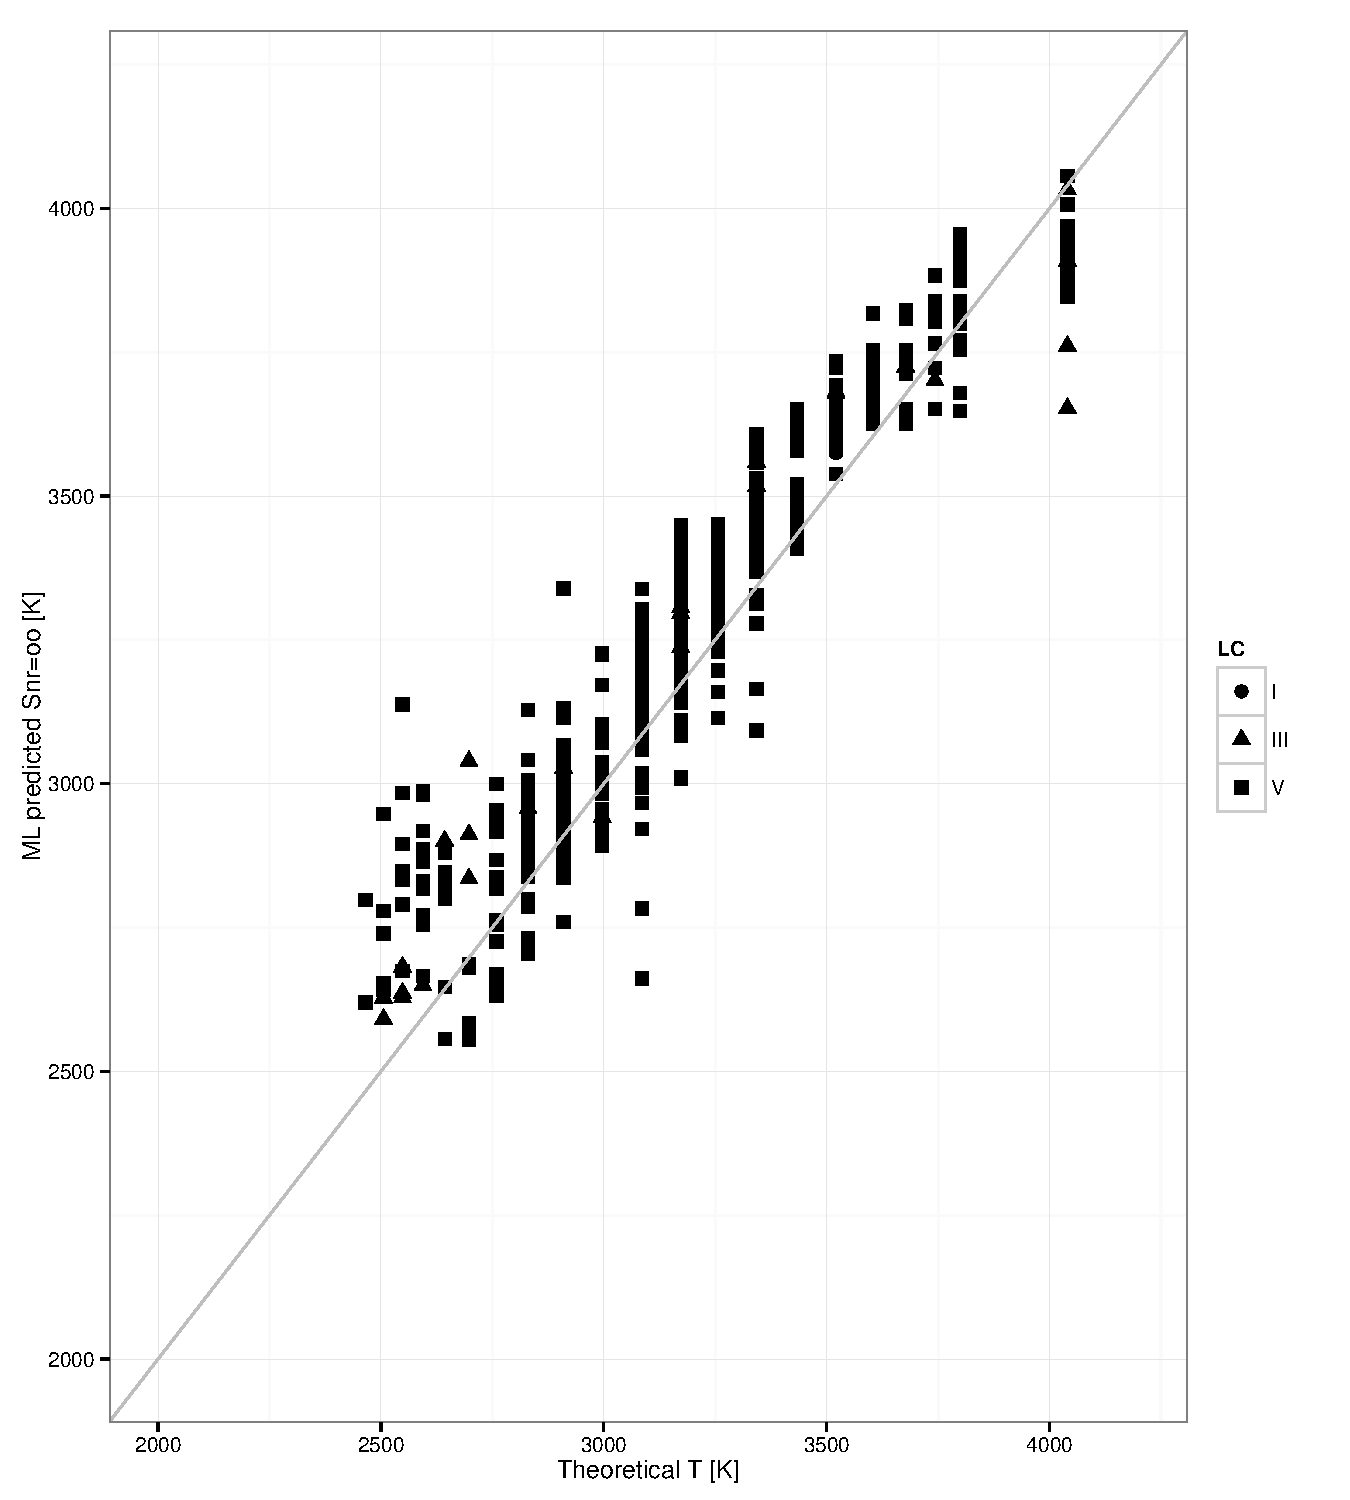
\includegraphics[width=11cm]{figs/ipac_T_ICAoo_LSB.pdf}
  \caption{Comparison between Temperature estimations from Theoretical Temperature 
  in x axis and the modeled ICA based estimation at SNR=$\infty$ on y-axis}
 \label{fig:ipac_icaoo_lsb}
 \end{subfigure}
  \begin{subfigure}{.35\textwidth}
  \centering
  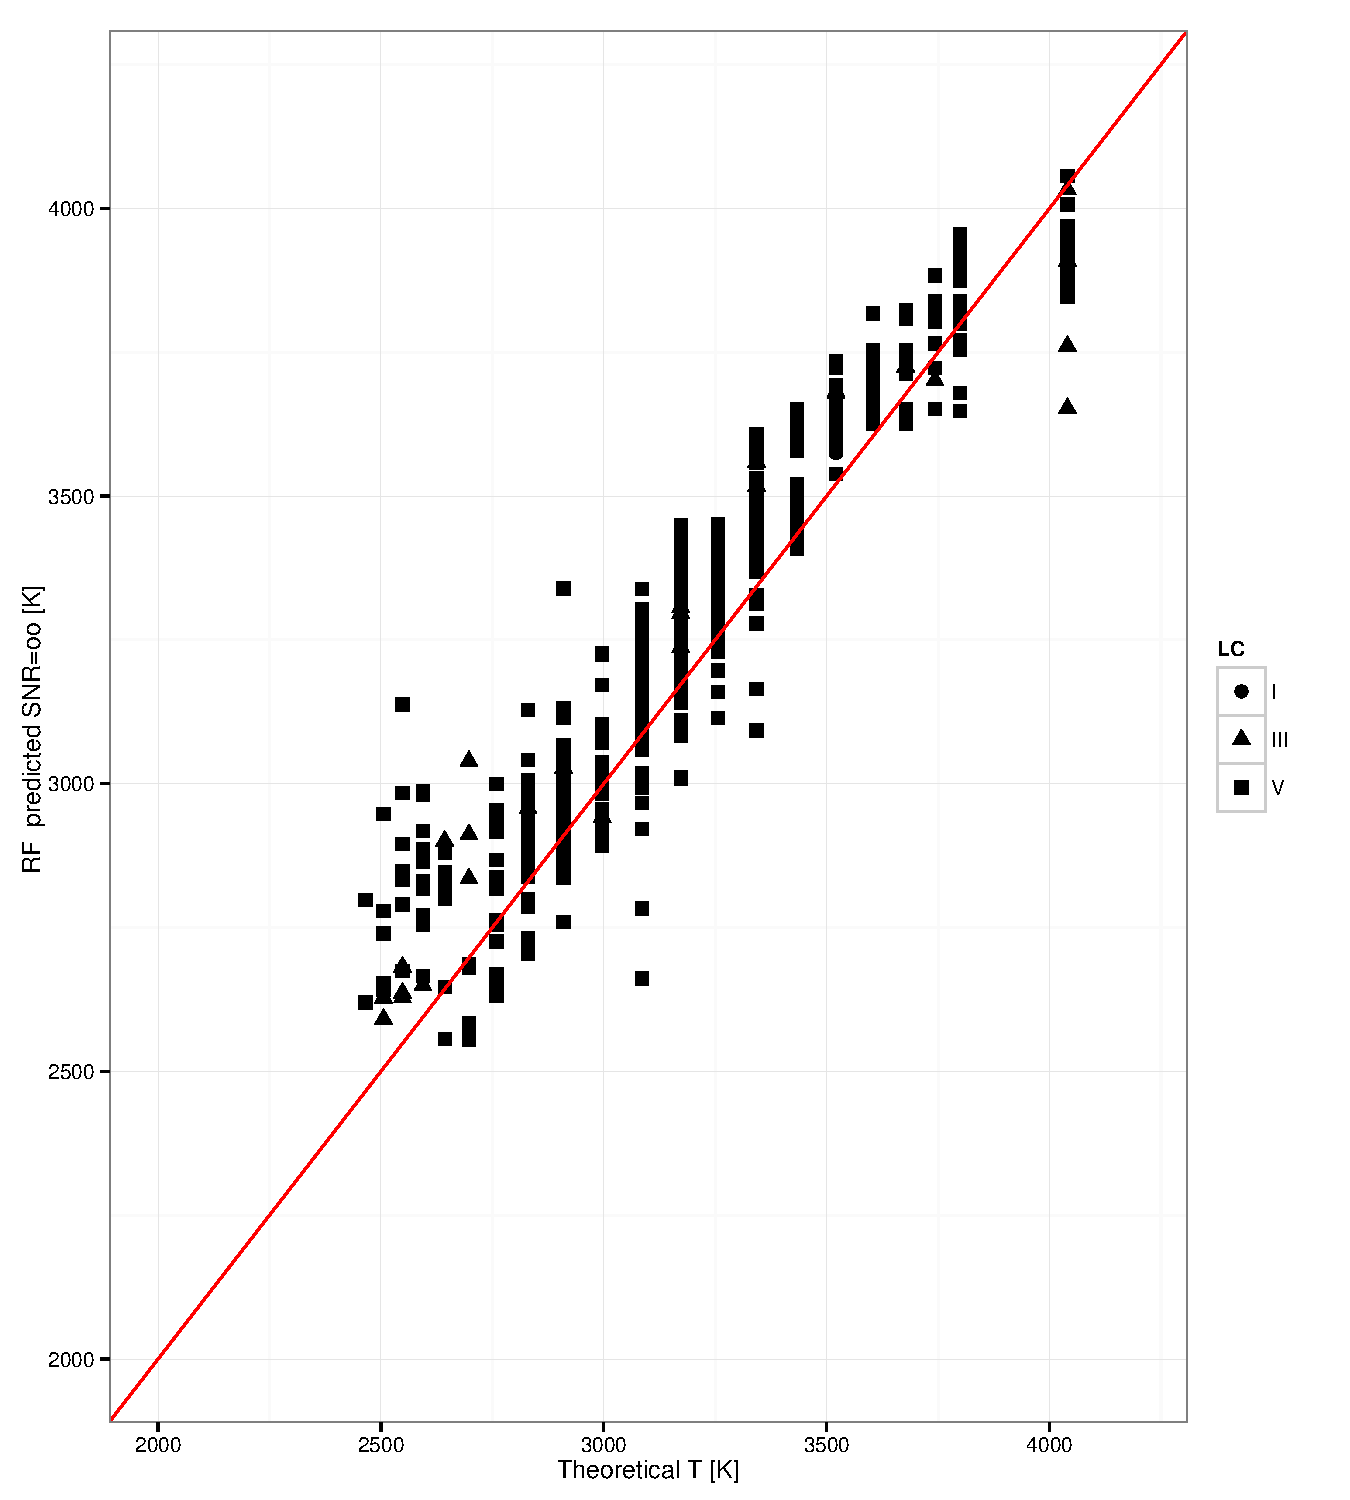
\includegraphics[width=11cm]{figs/ipac_T_RFoo_LSB.pdf}
  \caption{Comparison between Temperature estimations from Theoretical Temperature 
  in x axis and the featured based Random Forest modeled at SNR=$\infty$ on y-axis}
 \label{fig:ipac_rfoo_lsb}
 \end{subfigure}
  \begin{subfigure}{.35\textwidth}
  \centering
  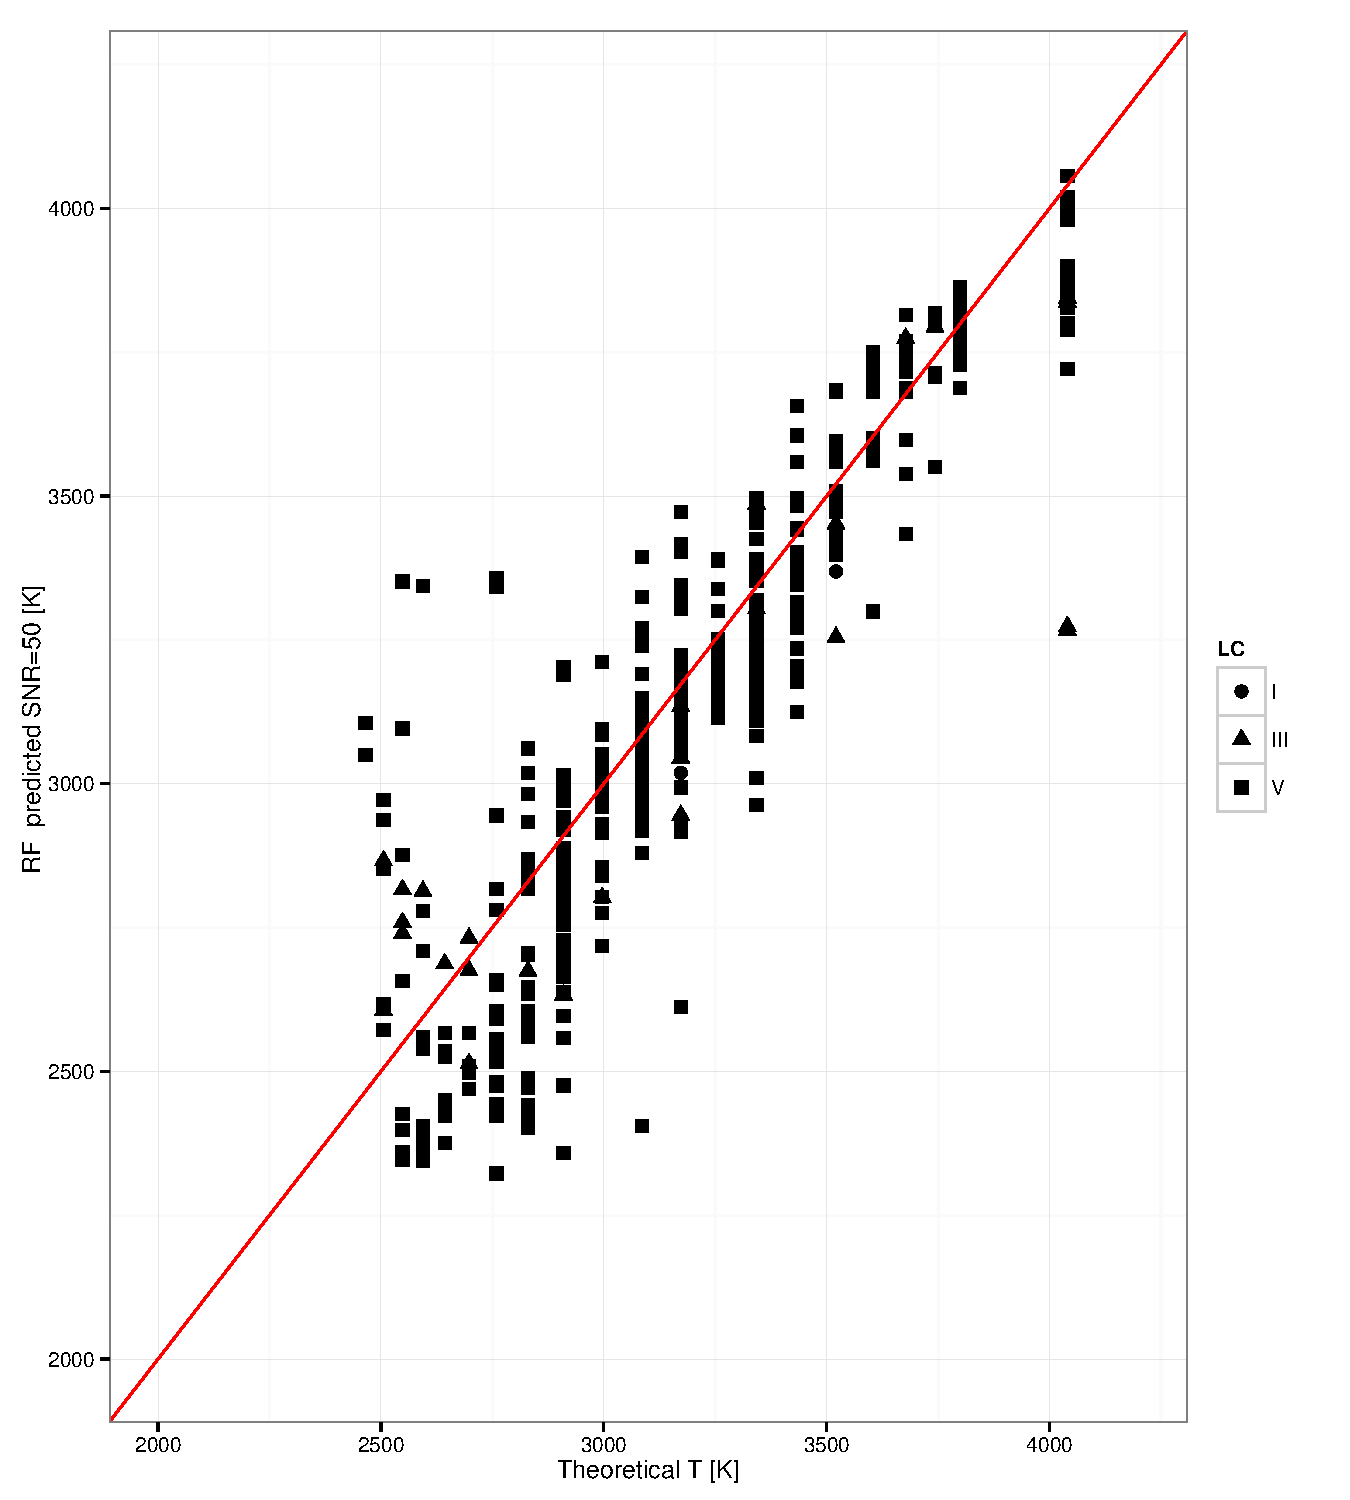
\includegraphics[width=11cm]{figs/ipac_T_RF50_LSB.pdf}
  \caption{Comparison between Temperature estimations from Theoretical Temperature 
  in x axis and the featured based Random Forest modeled at SNR=$50$ on y-axis}
 \label{fig:ipac_rf50_lsb}
 \end{subfigure}
 \label {fig:comp01}
 \caption{Performance comparison between the different strategies for Teperature prediction}
\end {figure*}

%%%%%%%%%%%%%%%%%%%%%%%%%%%%%%%%%%%%%%%%%%%%%%%%%%%%%%%%%%%%%%%
% Comparison with predictions from Cesetti's features. 
%%%%%%%%%%%%%%%%%%%%%%%%%%%%%%%%%%%%%%%%%%%%%%%%%%%%%%%%%%%%%%%

Having shown that the feature selection with GAs degrades the
performance of regression models, one can wonder whether a different
feature selection procedure would produce better results. In
particular, we investigate the possibility that the features proposed
by \cite{cesetti} result in a performance equal to or even better than
the one achieved with $\chi^2$.

%\begin{table}
%\begin{center}
%\begin{tabular}{rrrr}
%  \hline
%  $\lambda_1$ & $\lambda_2$ & $\lambda_{cont;1}$ & $\lambda_{cont;2} $ \\ 
%  \hline
%8461 & 8474 & 8474 & 8484 \\
%8484 & 8513 & 8474 & 8484 \\
%8522 &  8562 & 8474 & 8484 \\
%8577 & 8619 & 8563 & 8577 \\
%8642 & 8682 & 8619 & 8642 \\
%8730 & 8772 & 8700 & 8725 \\
%8802 & 8811 & 8776 & 8792 \\
%8850 & 8890 & 8815 & 8850 \\
%9000 & 9030 & 8983 & 8998 \\
%9080  & 9100 & 9040 & 9050 \\
%\hline
%\end{tabular}
%\caption {Features selected by following suggestions from Cesetti et al, table 1. } 
%\label{tab:tab_CS_T}
%\end{center}
%\end{table}

We train the same regression models applied to the GA selected
features, to the features selected in \cite{cesetti}, again learning
from BT-Settl spectra of various SNRs and predicting over the IPAC
set. A summary of the results can be found in Table
\ref{tab:tab_CS_Model}, where we use CS- to indicate that the model was
trained using the features by \cite{cesetti}.

\begin{table*}
\begin{center}
\begin{tabular}{@{}rrrcrrcrr@{}}\toprule
& \multicolumn{2}{c}{$SNR = 10$} & \phantom{ab}& \multicolumn{2}{c}{$SNR = 50$} &
\phantom{ab} & \multicolumn{2}{c}{$SNR = \infty$}\\
\cmidrule{2-3} \cmidrule{5-6} \cmidrule{8-9}
$Regression Models$ & $RMSE$ & $RMDSE$ && $RMSE$ & $RMDSE$     && $RMSE$       & $RMDSE$ \\ \midrule
CS-RF   & 203       & 140       && 243       & {\bf 121} &&  {\bf 306} &  {\bf 172}  \\
CS-GBM  & {\bf 188} & {\bf 120} && {\bf 161} & 138       &&  337       &  222  \\
CS-SVR  & 197       & 135       && 379       & 194       &&  840       &  688  \\
CS-NNET & 207       & 135       && 514       & 296       &&  719       &  489  \\
CS-MARS & 252       & 124       && 789       & 186       && 3464       &  784  \\
CS-KNN  & 235       & 158       && 246       & 137       &&  314       &  175  \\
CS-KPLS & 250       & 201       && 741       & 361       && 2247       & 1424  \\
CS-RR   & 211       & 128       && 400       & 239       &&  828       &  774  \\

\hline
\end{tabular}
\caption {Performances of regression models trained on the features
  selected by \cite{cesetti} applied to BT-Settl spectra.}
\label{tab:tab_CS_Model}
\end{center}
\end{table*}

For SNR=10, the GA best models (GA-KPLS in RMDSE or GA-RF in RMSE)
outperform the best CS model (GA-GBM). For SNR=50 the situation
depends on the figure-of-merit used to compare the classifiers: in
RMSE the best model is CS-GBM while in RMDSE GA-GBM outperforms all
CS-models. Finally, for the unrealistic case of noiseless spectra,
Table \ref{tab:tab_CS_Model} shows an overwhelming degradation of the
prediction accuracy from CS- features. {\bf Overfitting?} But even in
the only case where the CS features outperform those selected by the
GA, the performance is below the one achieved by the minimum-$\chi^2$
approach.

%%% HERE 1 %%%
The relationship between the GA predicted Temperature and the one
measured by Rojas-Ayala can be found in the
Figure~\ref{fig:ipac_lt_lt}
\begin{figure}
 \begin{center}
 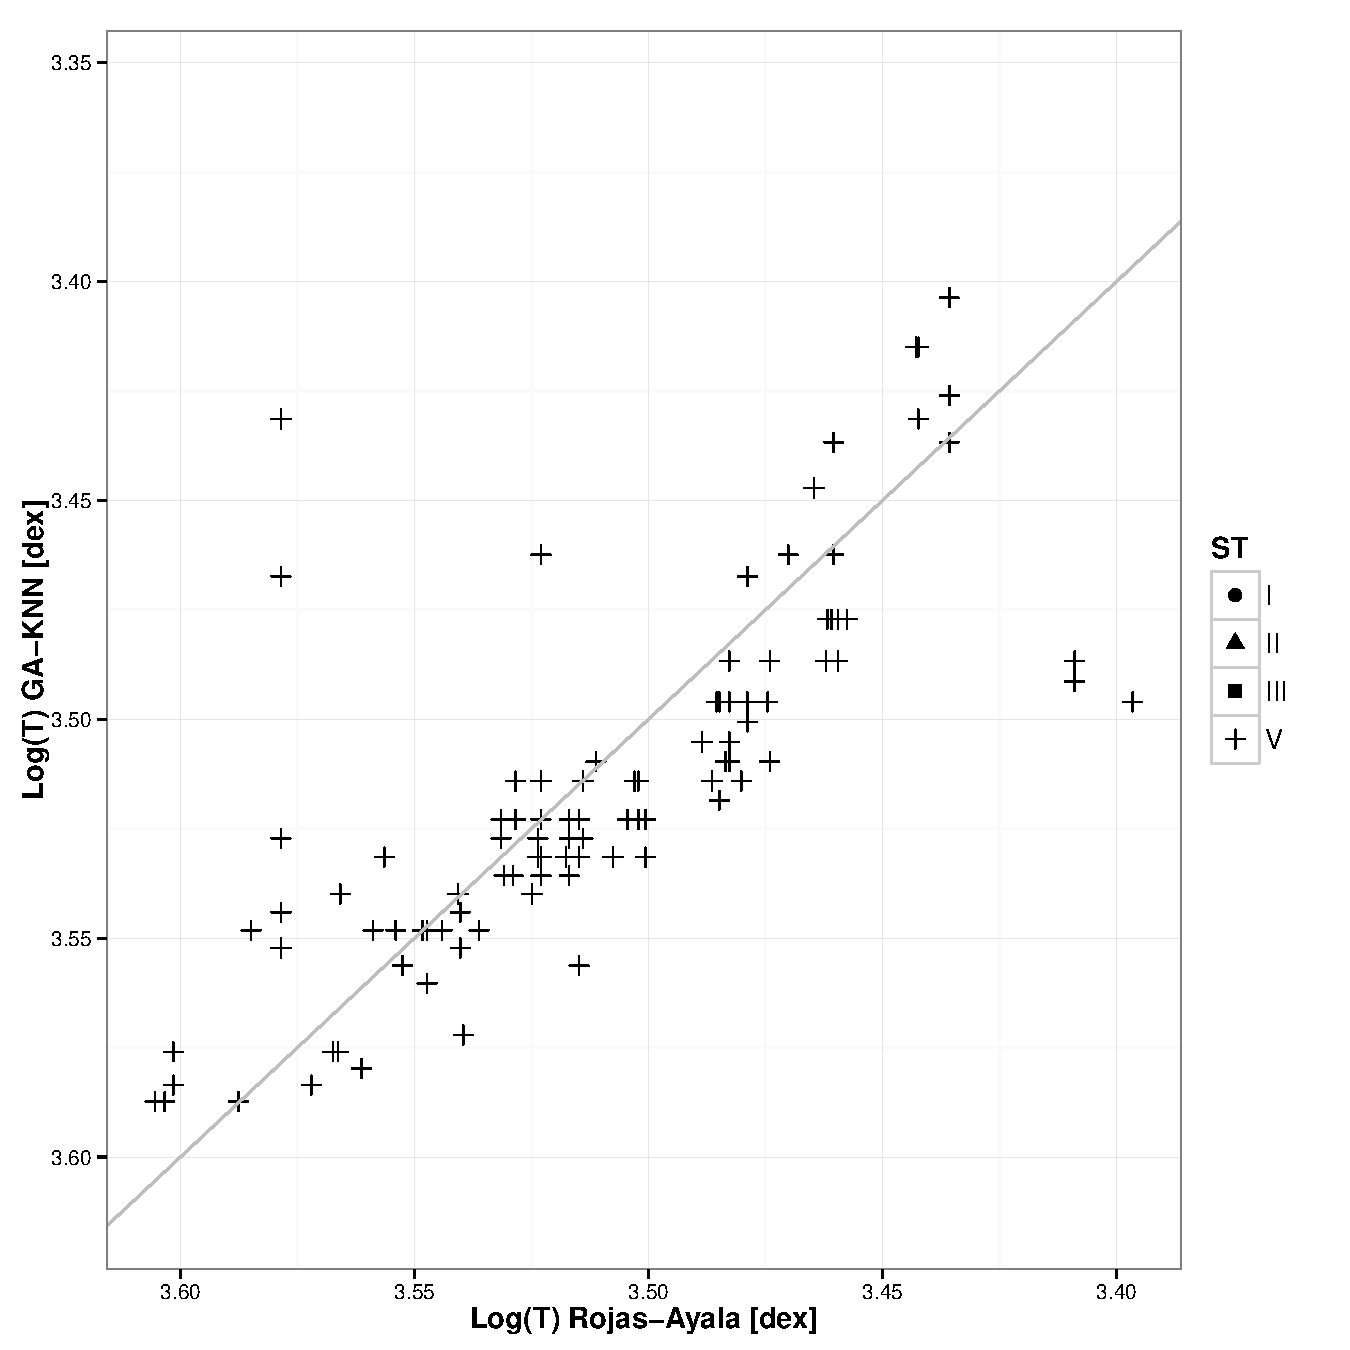
\includegraphics[width=12cm]{figs/ipac_LG_Trojas_Tknn_10.pdf}
 \caption{Relationship between $log(T) from Rojas-Ayala $ in the x axis 
 and $log(T)$ as predicted by KNN with SNR=$10$}
 \label{fig:ipac_lt_lt}
 \end{center}
\end{figure}
%%%%%%%%%%%%%

\subsubsection{Surface gravity models}

As in the IRTF exercise, we attempt to select features for surface
gravity estimation from BT-Settl spectra using GAs despite the much
lower spectral resolution and smaller wavelength coverage of the IPAC
spectra. Since there is no substantive compilation of surface
gravities that we could cross match with the IPAC list of M stars in
the Dwarf Archive, we are left with the same plausibility arguments
used in the IRTF study which are based on the $\log(T_{\rm
  eff})$--$\log(g)$ diagram.

We again use the effective temperatures as input of the regression
models. Table~\ref{tab:models_G_rmse} shows the cross-validation RMSE
and RMDSE for the same set of regression models used throughout this
article. It shows that the GA-RF model outperforms all other in all
SNR regimes, giving a consistent RMDSE of 1.0 dex. Obviously, this is
barely enough for classification in luminosity classes.

% HERE 2: This must be wrong: the Chi^2 and ICA columns are almost empty
% so I have asked Joaquín why. If the RMDSE are computed from these empty columns, these figures are just wrong.

\ra{1.3}
\begin{table*}\centering
\begin{tabular}{@{}rrrcrrcrr@{}}\toprule
& \multicolumn{2}{c}{$SNR = 10$} & \phantom{ab}& \multicolumn{2}{c}{$SNR = 50$} &
\phantom{ab} & \multicolumn{2}{c}{$SNR = \infty$}\\
\cmidrule{2-3} \cmidrule{5-6} \cmidrule{8-9}
$Regression Models$ & $RMSE$ & $RMDSE$ && $RMSE$ & $RMDSE$     && $RMSE$       & $RMDSE$ \\ \midrule
$\chi^2$    & 2.2       & 1.6       && 2.2       & 1.4       && 2.2       & 1.6 \\
PPR-ICA     & 2.1       & 1.8       && 1.8       & 1.4       && 4.3       & 4.2 \\
GA-RF       & {\bf 1.3} & {\bf 1.0} && {\bf 1.6} & {\bf 1.1} && {\bf 1.4} & {\bf 0.9} \\
GA-GBM      & 1.6       & 1.1       && 1.7       & 1.4       && 1.7       & 1.2 \\
GA-SVR      & 2.0       & 1.8       && 2.1       & 1.9       && 2.3       & 1.6 \\
GA-NNET     & 2.0       & 1.8       && 2.2       & 1.9       && 3.2       & 2.8 \\
GA-MARS     & 1.8       & 1.5       && 2.0       & 1.7       && 2.0       & 1.5 \\
GA-KNN      & 2.0       & 1.5       && 2.2       & 1.7       && 1.7       & 1.2 \\
GA-KPLS     & 1.8       & 1.4       && 2.0       & 1.7       && 2.7       & 2.3 \\
GA-RR       & 2.0       & 1.8       && 2.1       & 1.8       && 3.7       & 3.2 \\

\bottomrule
\end{tabular}
\caption {RMSE and RMDSE for the various regression models predicting $Log(G)$ [dex].} 
\label{tab:models_G_rmse} 
% \end{center}
\end{table*}

Figure \ref{fig:teffvsloggIPAC} shows the $\log(T_{\rm
  eff})$--$\log(g)$ diagram for the GA-RF and GA-NNET models. The
latter is, in our opinion, the one that shows the diagram that is most
with Fig. \ref{} in this work, and Fig. 1 in \cite{cesetti}. All GA-
models predict decreasing surface gravities for main sequence stars
below $\log(T_{\rm eff}=3.6$. GA-NNET predicts main sequence values
between $4 \le \log(g) \le6$, while luminosity classes III-I appear
clearly separated from the main sequence with values concentrated in
the 4-6 range except for the hottest cases with $\log(T_{rm eff} >
3.55$. The GA-RF results, despite showing the best cross-validation
errors (RMSE/RMDSE), result in unrealistic main sequence gravities. We
interpret this as the result of overfitting to the training examples. 

\begin{figure*}
 \begin{center}
 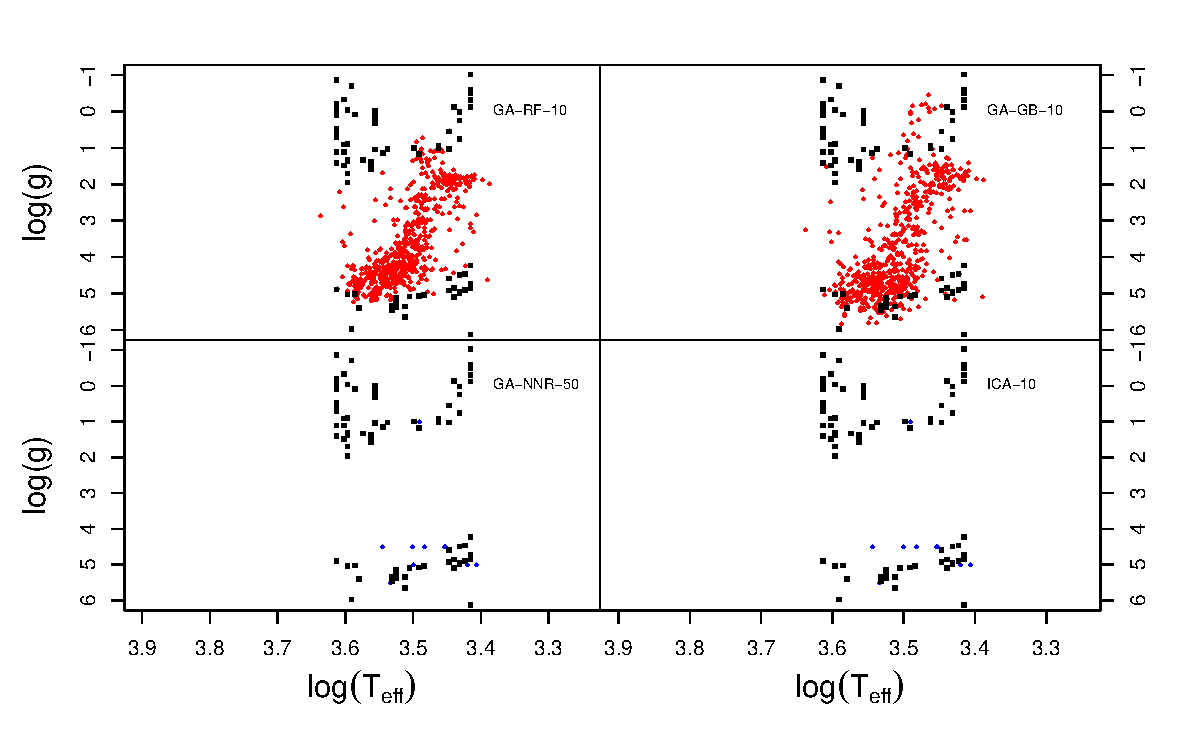
\includegraphics[width=12cm]{figs/ipac-teff-logg.pdf}
 \caption{Relationship between $log(T) $ ($x$ axis) 
 and $log(g)$ ($y$ axis) for several regression models.}
 \label{fig:teffvsloggIPAC}
 \end{center}
\end{figure*}

{\bf Right now, it appears that feature selected models are worse than $\chi^2$, judging only from the 10 available estimates (mail sent to jbmere). If so, the conclusion is clear: we should not do feature selection at these resolutions. This is useful as Cesseti et al do not question the utility of feature selection. For the IRTF (which is the dataset used by Cesseti et al), we should check this: are the models with feature selection better than $\chi^2$?}

\subsubsection{Metallicity models} 

Finally, the same analysis is performed for the Metalicty parameter, 
again by considering Temperature as a fixed feature.
In Table~\ref{tab:models_M_rmse} 
we can see the analysis of performance of different classes of
models and cosidering a variety in features. The checks were carried out against 
$Met$ from Neves III.

%
% Metalicidad teórica desde NevesIII para IPAC
%
\ra{1.3}
\begin{table*}\centering
\begin{tabular}{@{}rrrcrrcrr@{}}\toprule
& \multicolumn{2}{c}{$SNR = 10$} & \phantom{ab}& \multicolumn{2}{c}{$SNR = 50$} &
\phantom{ab} & \multicolumn{2}{c}{$SNR = \infty$}\\
\cmidrule{2-3} \cmidrule{5-6} \cmidrule{8-9}
$Regression Models$ & $RMSE$ & $RMDSE$ && $RMSE$ & $RMDSE$     && $RMSE$       & $RMDSE$ \\ \midrule
$\chi^2 BTSettl$    & 0.55    & 0.27   && 0.51 & 0.29 && 0.43  & 0.29 \\
$ ICA+ ppr$         & 0.48 & 0.27 && 0.70  & 0.39 && 0.85  & 0.71 \\
$rf $               & 0.55 & 0.38    && 0.71  & 0.61   && 0.23  & 0.16 \\
$gbm $              & 0.64 & 0.43 && 0.87  & 0.84  && 0.31  & 0.23 \\
$ svr $             & 0.46 & 0.26   && 0.57 & 0.44  && 3.38  & 2.33 \\
$ nnet $            & 0.52 & 0.45      && 0.66 & 0.54  && 2.03  & 1.88 \\
$ knn $             & 0.37  & 0.28   && 0.99  & 0.78 && 0.56 & 0.32 \\ 
$ mars+ bagging $   & 0.71  & 0.47 && 0.80   & 0.69   && 1.15    & 0.68 \\
$ pls $             & 0.67  & 0.61  && 0.63  & 0.55 && 1.17 & 1.02 \\ 
$Rule Regression $  & 0.47 & 0.29 && 0.50 & 0.36  && 1.18 &  1.18 \\

\bottomrule
\end{tabular}
\caption {RMSE and RMDSE for the various regression models predicting $Met$ [dex].} 
\label{tab:models_M_rmse} 
% \end{center}
\end{table*}


{\bf Noooo}
The relationship between the GA predicted Temperature and the one measured by Rojas-Ayala can be 
found in the Figure~\ref{fig:ipac_mt}
\begin{figure}
 \begin{center}
 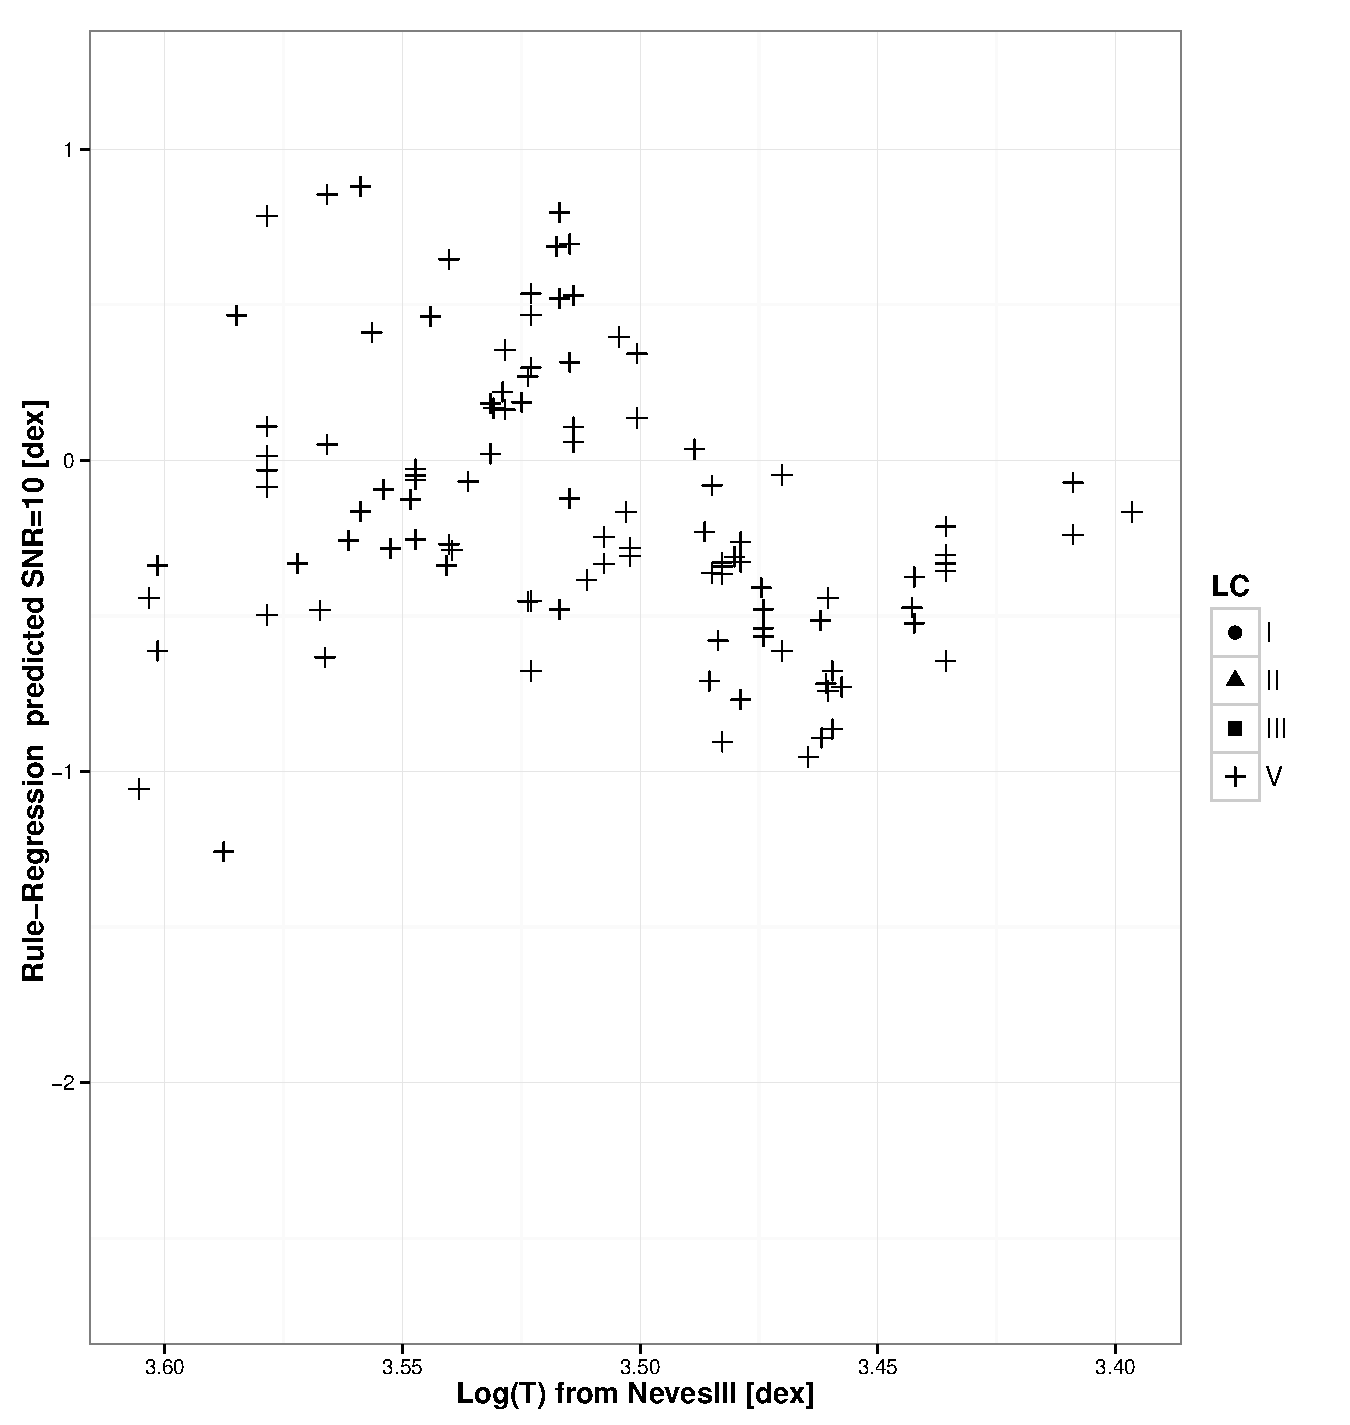
\includegraphics[width=12cm]{figs/ipac_Met_10_NevesIII.pdf}
 \caption{Relationship between $ T from NevesIII $ in the x axis 
 and $ Met $ as predicted by Regression Rules with SNR=$10$}
 \label{fig:ipac_mt}
 \end{center}
\end{figure}


% In Figure~\ref{fig:M_chi2_50_cesetti} and Figure~\ref{fig:M_GAM_1010_Cesetti} 
% relationships between metalicity predicted by global espectrum estimation 
% and GA feature based estimation against the real values
% provided by \cite{2013A&A...549A.129C} can be observed.

% \begin {figure}
%  \centering
%  \begin{subfigure}{.85\textwidth}
%   \centering
%   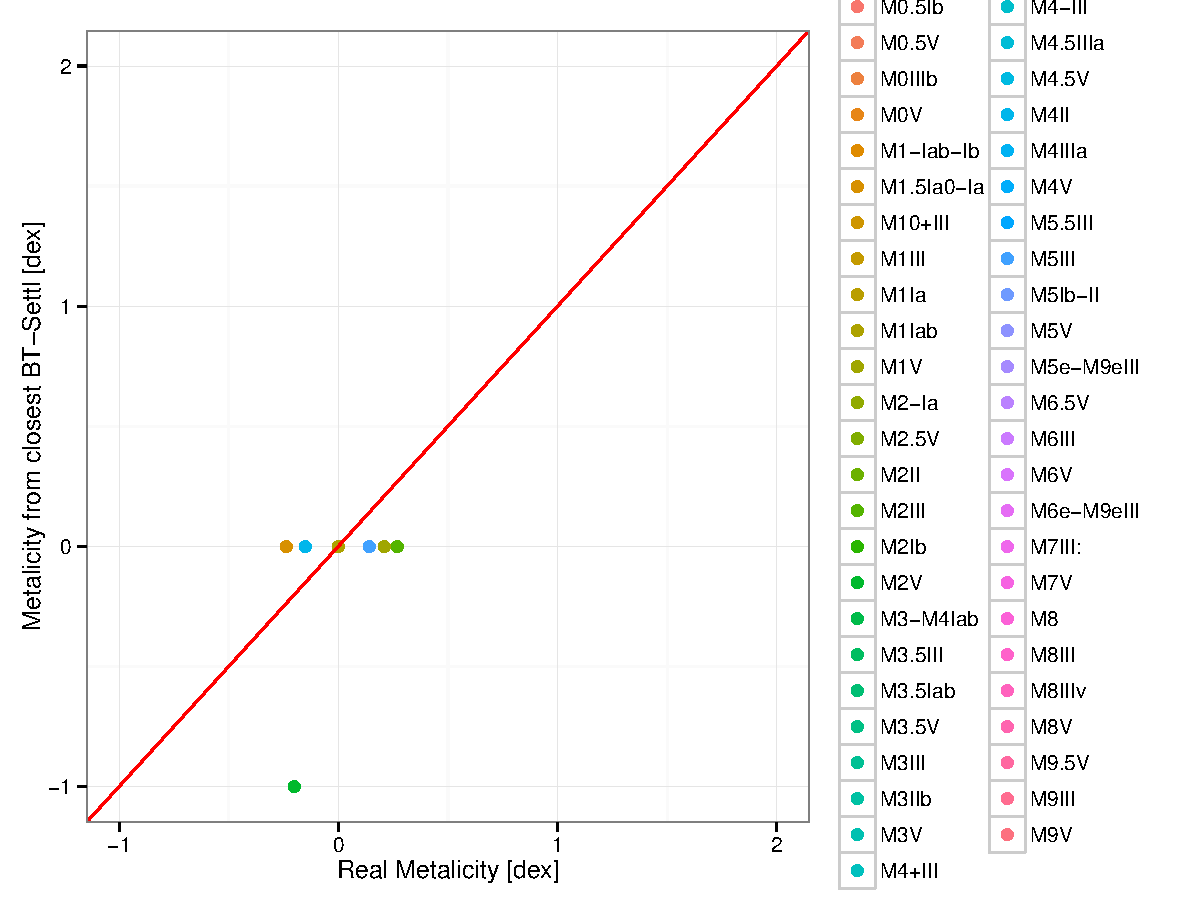
\includegraphics[width=12cm]{figs/M_Chi2_50_Cesetti.pdf}
%   \caption{Comparison between Metalicity estimations from Spectral Subtype 
%  in x axis and the closest BT\_Settl spectra by $\chi^2$ at SNR=$50$ on y-axis}
%  \label{M_chi2_50_cesetti}
%  \end{subfigure}
%   \begin{subfigure}{.85\textwidth}
%   \centering
%   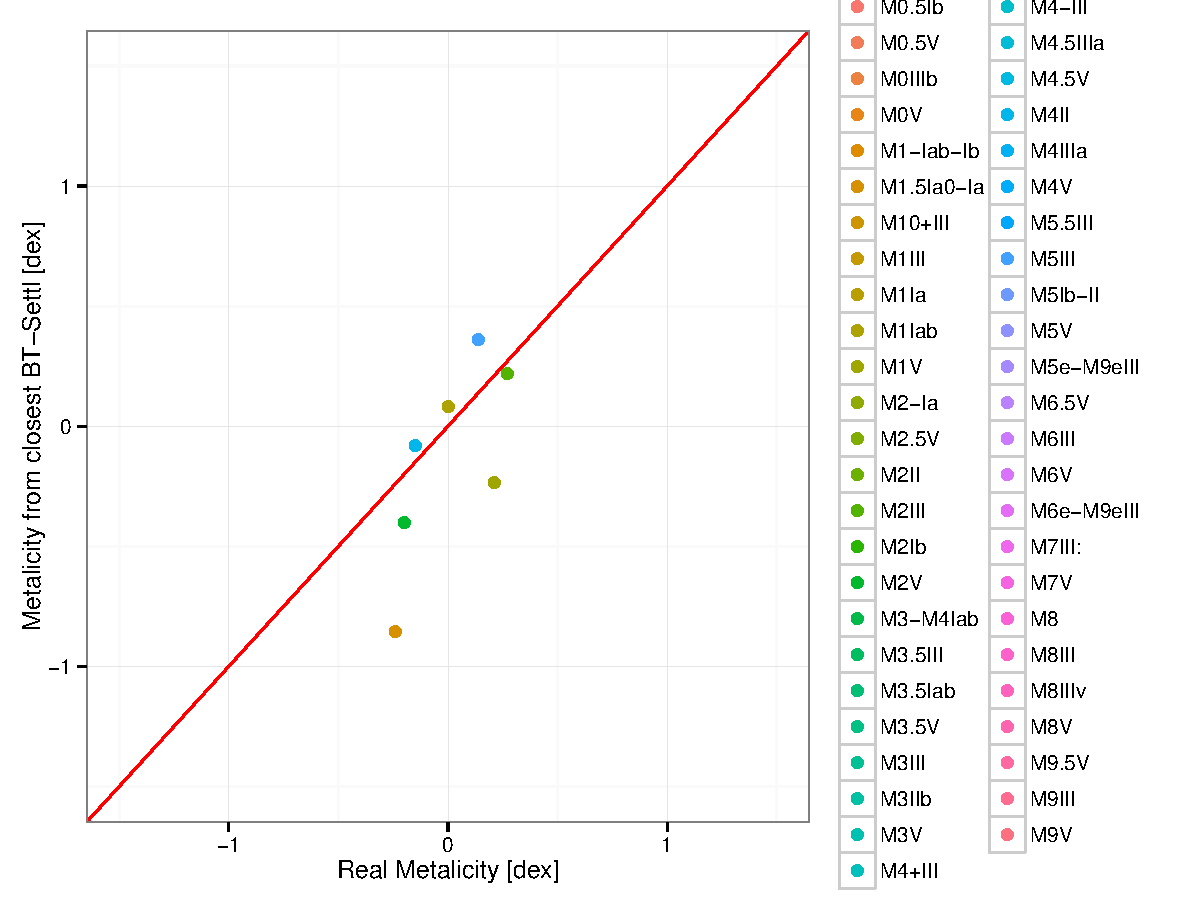
\includegraphics[width=12cm]{figs/M_GAM_1010_Cesetti.pdf}
%   \caption{Comparison between Metalicity estimations from Spectral Subtype 
%  in x axis and the Support Vector Machines for Ga based features trained with BT\_Settl 
%  at SNR=$\infty$ and features for forecasting at SNR=$\infty$ on y-axis}
%  \label{fig:M_GAM_1010_Cesetti}
%  \end{subfigure}
%  \label {fig:comp03}
%  \caption{Performance comparison between the $chi^2$ based selection 
%           and the band oriented features to forecast Log(g)}
% \end {figure}
%
   
   

% De nuevo, el análisis y discusión, función de lo que queramos dejar

